\documentclass{standalone}
\usepackage{tikz}
\usepackage{pgfplots}

\pgfplotsset{compat = newest}
\definecolor{lessgreen}{RGB}{0,100,0}
\begin{document}
    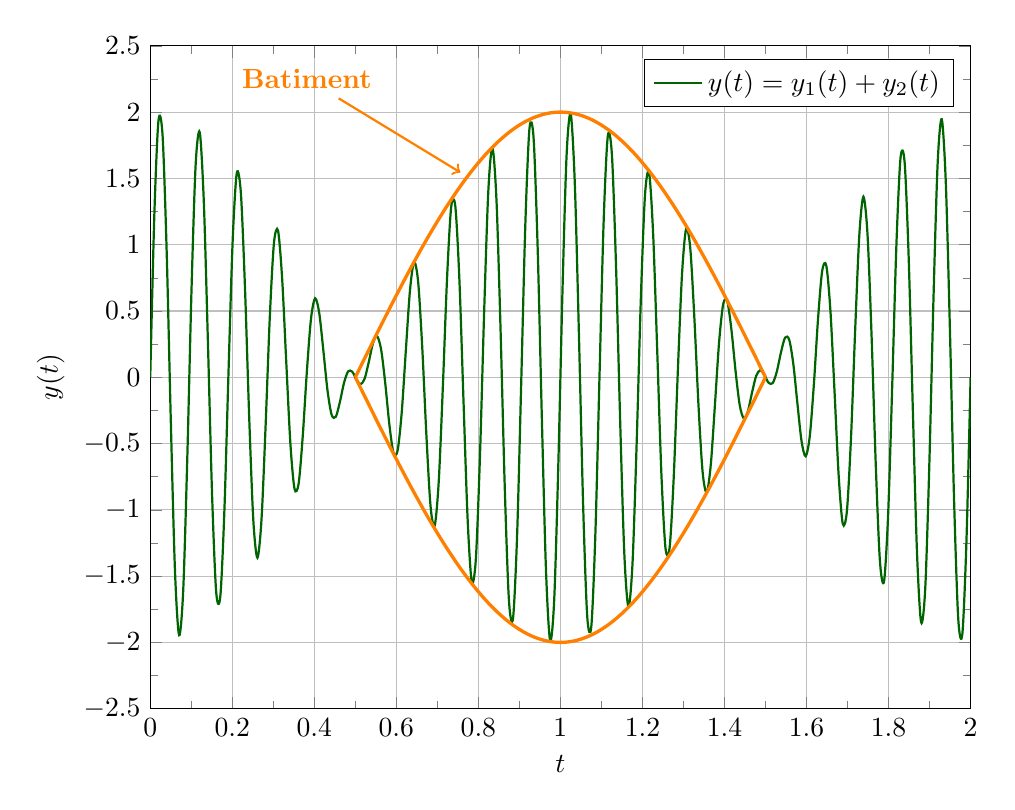
\begin{tikzpicture}
        \begin{axis}[
            xmin = 0, xmax = 2, %
            ymin = -2.5, ymax = 2.5, %
            xtick distance = 0.2, %Is the distance between major ticks in the x-axis.
            ytick distance = 0.5, %Is the distance between major ticks in the y-axis.
            grid = major, %When this options is set to both the minor and major grid are plotted.
            minor tick num = 1, %Is the number of ticks between major ticks.
            major grid style = {lightgray}, %Changes the color and stroke of the major grid.
            width = 12cm, %sets the width of the figure
            height = 10cm,  %sets the height of the figure
            xlabel = {$t$}, %
            ylabel = {$y(t)$}, %
            legend cell align = {left}, %
        ]
            \addplot[
                domain=0:2, %Domain of the fucntion
                samples=200, %This parameter determines the number of point to be plotted for the function, while bigger the number better looks the function.
                smooth, %f we use this option, the compiler makes an interpolation between the point plotted to get a soft appearance for the function.
                thick, %Stroke of the function. Options: ultra thin, very thin, thin, semithick, thick, very thick, ultra thick.
                lessgreen %Color of the function.
            ]{2*cos(2*pi*0.5*deg(x))*sin(2*pi*10.5*deg(x))};
            \addplot[
                domain=0.5:1.5, %Domain of the fucntion
                samples=200, %This parameter determines the number of point to be plotted for the function, while bigger the number better looks the function.
                smooth, %f we use this option, the compiler makes an interpolation between the point plotted to get a soft appearance for the function.
                very thick, %Stroke of the function. Options: ultra thin, very thin, thin, semithick, thick, very thick, ultra thick.
                orange %Color of the function.
            ]{2*cos(2*pi*0.5*deg(x))};
            \addplot[
                domain=0.5:1.5, %Domain of the fucntion
                samples=200, %This parameter determines the number of point to be plotted for the function, while bigger the number better looks the function.
                smooth, %f we use this option, the compiler makes an interpolation between the point plotted to get a soft appearance for the function.
                very thick, %Stroke of the function. Options: ultra thin, very thin, thin, semithick, thick, very thick, ultra thick.
                orange %Color of the function
            ]{-2*cos(2*pi*0.5*deg(x))};
            \node [anchor=west,color=orange,font=\bf] (source) at (axis cs:0.2,2.25){Batiment};
            \node (destination) at (axis cs:0.78,1.5){};
            \draw[->,color=orange,thick](source)--(destination);
            \legend{$y(t)=y_1(t)+y_2(t)$}
        \end{axis}
    \end{tikzpicture}
\end{document}